\documentclass{report}
\usepackage{amsmath}
\usepackage{pgf}
\usepackage{graphicx}
\usepackage{tikz}
\usepackage{pgfplots}

\begin{document}
\title{Sorting Algorithms}
\author{Philip J.Y. Lee}
\maketitle

\chapter{1}
\section{Introduction to Sorting Algorithms}
\subsection{Insertion Sort}
Insertion sort is a kind of sort that...
\subsection{Merge Sort}
Merger sort is a kind of sort that...
\subsection{Heap Sort}
Heap sort is a kind of sort that...
\subsection{Quick Sort}
Quick sort is a kind of sort that...

\chapter{2}
% GRAPHICS
%==========For Failure===========

 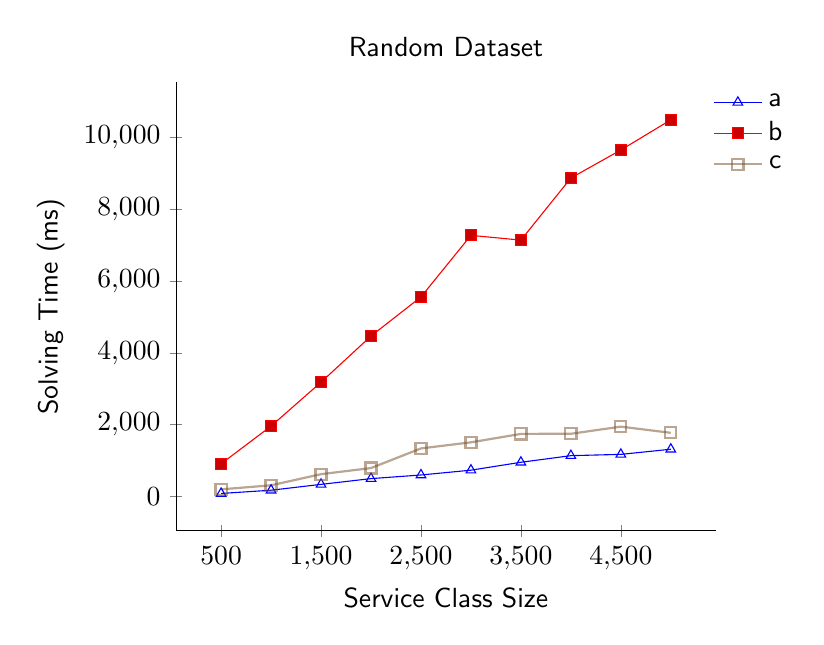
\begin{tikzpicture}[font=\sffamily]
 \begin{axis}[title=Random Dataset,
                              legend pos=outer north east,
                              legend style={draw=none},
                              xtick={500,1500,...,5000}, % new bit
                              scaled ticks=false,
                              log ticks with fixed point={1000 sep=},
                              axis x line=bottom,
                              axis y line=left,
                              axis line style=-,
                              minor tick style={draw=none},
                              enlargelimits,
                              ylabel = Solving Time (ms),
                              xlabel = Service Class Size,
                              every axis legend/.append style={xshift=-10pt}
                              ]
 \addplot+[mark=triangle] plot coordinates{(500,88)(1000,178)(1500,341)(2000,501)(2500,602)(3000,736)(3500,956)(4000,1140)(4500,1176)(5000,1319)};
 \addplot plot coordinates{(500,913)(1000,1963)(1500,3185)(2000,4470)(2500,5558)(3000,7273)(3500,7140)(4000,8869)(4500,9648)(5000,10488)};
 \addplot+[draw opacity=0.5, thick, mark=square] plot coordinates{(500,202)(1000,315)(1500,625)(2000,795)(2500,1342)(3000,1511)(3500,1746)(4000,1749)(4500,1948)(5000,1776)};
 \legend{a, b, c}
 \end{axis}
 \end{tikzpicture}

 %==========For Failure===========





\end{document}
